% Options for packages loaded elsewhere
\PassOptionsToPackage{unicode}{hyperref}
\PassOptionsToPackage{hyphens}{url}
\documentclass[
]{article}
\usepackage{xcolor}
\usepackage[margin=1in]{geometry}
\usepackage{amsmath,amssymb}
\setcounter{secnumdepth}{-\maxdimen} % remove section numbering
\usepackage{iftex}
\ifPDFTeX
  \usepackage[T1]{fontenc}
  \usepackage[utf8]{inputenc}
  \usepackage{textcomp} % provide euro and other symbols
\else % if luatex or xetex
  \usepackage{unicode-math} % this also loads fontspec
  \defaultfontfeatures{Scale=MatchLowercase}
  \defaultfontfeatures[\rmfamily]{Ligatures=TeX,Scale=1}
\fi
\usepackage{lmodern}
\ifPDFTeX\else
  % xetex/luatex font selection
\fi
% Use upquote if available, for straight quotes in verbatim environments
\IfFileExists{upquote.sty}{\usepackage{upquote}}{}
\IfFileExists{microtype.sty}{% use microtype if available
  \usepackage[]{microtype}
  \UseMicrotypeSet[protrusion]{basicmath} % disable protrusion for tt fonts
}{}
\makeatletter
\@ifundefined{KOMAClassName}{% if non-KOMA class
  \IfFileExists{parskip.sty}{%
    \usepackage{parskip}
  }{% else
    \setlength{\parindent}{0pt}
    \setlength{\parskip}{6pt plus 2pt minus 1pt}}
}{% if KOMA class
  \KOMAoptions{parskip=half}}
\makeatother
\usepackage{color}
\usepackage{fancyvrb}
\newcommand{\VerbBar}{|}
\newcommand{\VERB}{\Verb[commandchars=\\\{\}]}
\DefineVerbatimEnvironment{Highlighting}{Verbatim}{commandchars=\\\{\}}
% Add ',fontsize=\small' for more characters per line
\usepackage{framed}
\definecolor{shadecolor}{RGB}{248,248,248}
\newenvironment{Shaded}{\begin{snugshade}}{\end{snugshade}}
\newcommand{\AlertTok}[1]{\textcolor[rgb]{0.94,0.16,0.16}{#1}}
\newcommand{\AnnotationTok}[1]{\textcolor[rgb]{0.56,0.35,0.01}{\textbf{\textit{#1}}}}
\newcommand{\AttributeTok}[1]{\textcolor[rgb]{0.13,0.29,0.53}{#1}}
\newcommand{\BaseNTok}[1]{\textcolor[rgb]{0.00,0.00,0.81}{#1}}
\newcommand{\BuiltInTok}[1]{#1}
\newcommand{\CharTok}[1]{\textcolor[rgb]{0.31,0.60,0.02}{#1}}
\newcommand{\CommentTok}[1]{\textcolor[rgb]{0.56,0.35,0.01}{\textit{#1}}}
\newcommand{\CommentVarTok}[1]{\textcolor[rgb]{0.56,0.35,0.01}{\textbf{\textit{#1}}}}
\newcommand{\ConstantTok}[1]{\textcolor[rgb]{0.56,0.35,0.01}{#1}}
\newcommand{\ControlFlowTok}[1]{\textcolor[rgb]{0.13,0.29,0.53}{\textbf{#1}}}
\newcommand{\DataTypeTok}[1]{\textcolor[rgb]{0.13,0.29,0.53}{#1}}
\newcommand{\DecValTok}[1]{\textcolor[rgb]{0.00,0.00,0.81}{#1}}
\newcommand{\DocumentationTok}[1]{\textcolor[rgb]{0.56,0.35,0.01}{\textbf{\textit{#1}}}}
\newcommand{\ErrorTok}[1]{\textcolor[rgb]{0.64,0.00,0.00}{\textbf{#1}}}
\newcommand{\ExtensionTok}[1]{#1}
\newcommand{\FloatTok}[1]{\textcolor[rgb]{0.00,0.00,0.81}{#1}}
\newcommand{\FunctionTok}[1]{\textcolor[rgb]{0.13,0.29,0.53}{\textbf{#1}}}
\newcommand{\ImportTok}[1]{#1}
\newcommand{\InformationTok}[1]{\textcolor[rgb]{0.56,0.35,0.01}{\textbf{\textit{#1}}}}
\newcommand{\KeywordTok}[1]{\textcolor[rgb]{0.13,0.29,0.53}{\textbf{#1}}}
\newcommand{\NormalTok}[1]{#1}
\newcommand{\OperatorTok}[1]{\textcolor[rgb]{0.81,0.36,0.00}{\textbf{#1}}}
\newcommand{\OtherTok}[1]{\textcolor[rgb]{0.56,0.35,0.01}{#1}}
\newcommand{\PreprocessorTok}[1]{\textcolor[rgb]{0.56,0.35,0.01}{\textit{#1}}}
\newcommand{\RegionMarkerTok}[1]{#1}
\newcommand{\SpecialCharTok}[1]{\textcolor[rgb]{0.81,0.36,0.00}{\textbf{#1}}}
\newcommand{\SpecialStringTok}[1]{\textcolor[rgb]{0.31,0.60,0.02}{#1}}
\newcommand{\StringTok}[1]{\textcolor[rgb]{0.31,0.60,0.02}{#1}}
\newcommand{\VariableTok}[1]{\textcolor[rgb]{0.00,0.00,0.00}{#1}}
\newcommand{\VerbatimStringTok}[1]{\textcolor[rgb]{0.31,0.60,0.02}{#1}}
\newcommand{\WarningTok}[1]{\textcolor[rgb]{0.56,0.35,0.01}{\textbf{\textit{#1}}}}
\usepackage{graphicx}
\makeatletter
\newsavebox\pandoc@box
\newcommand*\pandocbounded[1]{% scales image to fit in text height/width
  \sbox\pandoc@box{#1}%
  \Gscale@div\@tempa{\textheight}{\dimexpr\ht\pandoc@box+\dp\pandoc@box\relax}%
  \Gscale@div\@tempb{\linewidth}{\wd\pandoc@box}%
  \ifdim\@tempb\p@<\@tempa\p@\let\@tempa\@tempb\fi% select the smaller of both
  \ifdim\@tempa\p@<\p@\scalebox{\@tempa}{\usebox\pandoc@box}%
  \else\usebox{\pandoc@box}%
  \fi%
}
% Set default figure placement to htbp
\def\fps@figure{htbp}
\makeatother
\setlength{\emergencystretch}{3em} % prevent overfull lines
\providecommand{\tightlist}{%
  \setlength{\itemsep}{0pt}\setlength{\parskip}{0pt}}
\usepackage{booktabs}
\usepackage{longtable}
\usepackage{array}
\usepackage{multirow}
\usepackage{wrapfig}
\usepackage{float}
\usepackage{colortbl}
\usepackage{pdflscape}
\usepackage{tabu}
\usepackage{threeparttable}
\usepackage{threeparttablex}
\usepackage[normalem]{ulem}
\usepackage{makecell}
\usepackage{xcolor}
\usepackage{bookmark}
\IfFileExists{xurl.sty}{\usepackage{xurl}}{} % add URL line breaks if available
\urlstyle{same}
% fallback for those not using the hyperref driver hyperxmp:
\makeatletter
\@ifundefined{xmpquote}{\newcommand{\xmpquote}[1]{#1}}{}
\makeatother
\hypersetup{
  pdftitle={\_02\_Analytical\_Tests\_Finalized},
  pdfauthor={ACT},
  hidelinks,
  pdfcreator={LaTeX via pandoc}}

\title{\_02\_Analytical\_Tests\_Finalized}
\author{ACT}
\date{2026-10-28}

\begin{document}
\maketitle

\section{0. Setup \& Data Ingestion}\label{setup-data-ingestion}

\subsection{0.1 Libraries}\label{libraries}

\begin{Shaded}
\begin{Highlighting}[]
\FunctionTok{library}\NormalTok{(dplyr)       }\CommentTok{\# Data manipulation}
\FunctionTok{library}\NormalTok{(stringr)     }\CommentTok{\# String manipulation}
\FunctionTok{library}\NormalTok{(tidyr)       }\CommentTok{\# Data pivoting}
\FunctionTok{library}\NormalTok{(readr)       }\CommentTok{\# Reading data}
\FunctionTok{library}\NormalTok{(kableExtra)  }\CommentTok{\# HTML Table formatting}
\FunctionTok{library}\NormalTok{(ggplot2)     }\CommentTok{\# Visualizations}
\FunctionTok{library}\NormalTok{(ggpubr)      }\CommentTok{\# Publication{-}ready plots}
\FunctionTok{library}\NormalTok{(rstatix)     }\CommentTok{\# T{-}tests and effect sizes}
\FunctionTok{library}\NormalTok{(broom)       }\CommentTok{\# Tidy statistical outputs}
\FunctionTok{library}\NormalTok{(forcats)     }\CommentTok{\# Factor manipulation}
\FunctionTok{library}\NormalTok{(effectsize)  }\CommentTok{\# effect size \& omega squared}
\end{Highlighting}
\end{Shaded}

\section{Data From Ingestion - Load \&
Analyze}\label{data-from-ingestion---load-analyze}

\begin{itemize}
\tightlist
\item
  \textbf{Reiterating Scales Info}

  \begin{itemize}
  \tightlist
  \item
    Stress Scale: \textbf{PSS} - \emph{Perceived Stress Scale} - 10
    Questions

    \begin{itemize}
    \tightlist
    \item
      Scoring: PSS scores are obtained by reversing responses (e.g., 0 =
      4, 1 = 3, 2 = 2, 3 = 1 \& 4 = 0) to the four positively stated
      items (items 4, 5, 7, \& 8) and then summing across all scale
      items. A short 4 item scale can be made from questions 2, 4, 5 and
      10 of the PSS 10 item scale.
    \end{itemize}
  \item
    SEFF Scale: \textbf{EFF} - \emph{Eearly Intervention Parent Self
    Efficacy} - 16 Questions

    \begin{itemize}
    \tightlist
    \item
      \textbf{Scoring Guidelines (Guimond et al., 2008):}

      \begin{itemize}
      \tightlist
      \item
        Mean/Total scores are computed by aggregating all items of the
        specific scale.
      \item
        Reverse Scored Items: 3, 5, 6, 8, 10, 12, 13, 15, 16.
      \item
        Parent Outcome Expectations: 3, 4, 5, 6, 7, 8, 10, 12, 15, 16.
      \item
        Parent Competence: 1, 2, 9, 14.
      \end{itemize}
    \end{itemize}
  \end{itemize}
\end{itemize}

\section{1. Load Ingested Tables
Files}\label{load-ingested-tables-files}

\begin{Shaded}
\begin{Highlighting}[]
\FunctionTok{load}\NormalTok{(}\AttributeTok{file =} \StringTok{"../\_output/Analytic\_Tables\_Finalize\_2026{-}10.Rdata"}\NormalTok{, }\AttributeTok{verbose =} \ConstantTok{TRUE}\NormalTok{)}
\end{Highlighting}
\end{Shaded}

\begin{verbatim}
## Loading objects:
##   CCMHC_Study_Data_Finalized
##   CCMHC_Study_Scores_Finalized
\end{verbatim}

\subsection{Include Only Complete
Cases}\label{include-only-complete-cases}

\begin{Shaded}
\begin{Highlighting}[]
\CommentTok{\# Data screening and complete{-}case flag}
\NormalTok{CCMHC\_Study\_Scores\_Finalized }\OtherTok{\textless{}{-}}\NormalTok{ CCMHC\_Study\_Scores\_Finalized }\SpecialCharTok{|\textgreater{}} 
  \FunctionTok{mutate}\NormalTok{(}\AttributeTok{Complete\_Case =} \SpecialCharTok{!}\FunctionTok{is.na}\NormalTok{(POST.PSS.sum) }\SpecialCharTok{\&} \SpecialCharTok{!}\FunctionTok{is.na}\NormalTok{(POST.EFF.sum))}

\FunctionTok{table}\NormalTok{(CCMHC\_Study\_Scores\_Finalized}\SpecialCharTok{$}\NormalTok{Group\_Assignment, CCMHC\_Study\_Scores\_Finalized}\SpecialCharTok{$}\NormalTok{Complete\_Case)}
\end{Highlighting}
\end{Shaded}

\begin{verbatim}
##               
##                FALSE TRUE
##   Control          2    5
##   Intervention     1   23
\end{verbatim}

\subsection{Make Specific Analytic
Tables}\label{make-specific-analytic-tables}

\begin{Shaded}
\begin{Highlighting}[]
\NormalTok{CCMHC\_Study\_Scores\_Finalized }\OtherTok{\textless{}{-}}\NormalTok{ CCMHC\_Study\_Scores\_Finalized }\SpecialCharTok{|\textgreater{}} \FunctionTok{filter}\NormalTok{(Complete\_Case}\SpecialCharTok{==}\ConstantTok{TRUE}\NormalTok{)}


\NormalTok{PSS }\OtherTok{\textless{}{-}}\NormalTok{ CCMHC\_Study\_Scores\_Finalized }\SpecialCharTok{|\textgreater{}} \FunctionTok{select}\NormalTok{(Study\_ID, Group\_Assignment, }\FunctionTok{contains}\NormalTok{(}\StringTok{"PSS"}\NormalTok{))}
\NormalTok{EFF }\OtherTok{\textless{}{-}}\NormalTok{ CCMHC\_Study\_Scores\_Finalized }\SpecialCharTok{|\textgreater{}} \FunctionTok{select}\NormalTok{(Study\_ID, Group\_Assignment, }\FunctionTok{contains}\NormalTok{(}\StringTok{"EFF"}\NormalTok{))}
\end{Highlighting}
\end{Shaded}

\begin{Shaded}
\begin{Highlighting}[]
\FunctionTok{library}\NormalTok{(tableone)}
\NormalTok{study.t1.pre }\OtherTok{\textless{}{-}} 
\NormalTok{  CCMHC\_Study\_Scores\_Finalized }\SpecialCharTok{\%\textgreater{}\%} 
\NormalTok{tableone}\SpecialCharTok{::}\FunctionTok{CreateTableOne}\NormalTok{(}
  \AttributeTok{vars =} \FunctionTok{c}\NormalTok{(}\StringTok{"PRE.PSS.sum"}\NormalTok{, }\StringTok{"PRE.PSS.mean"}\NormalTok{, }\StringTok{"PRE.EFF.sum"}\NormalTok{, }\StringTok{"PRE.EFF.mean"}\NormalTok{),}
  \AttributeTok{strata =} \StringTok{"Group\_Assignment"}\NormalTok{,}
  \AttributeTok{factorVars =} \FunctionTok{c}\NormalTok{(}\StringTok{"Group\_Assignment"}\NormalTok{),}
  \AttributeTok{testNormal =} \StringTok{"oneway.test"}
\NormalTok{) }
\NormalTok{study.t1.pre }\SpecialCharTok{\%\textgreater{}\%}   \FunctionTok{print}\NormalTok{(}\AttributeTok{showAllLevels =} \ConstantTok{TRUE}\NormalTok{, }\AttributeTok{quote =} \ConstantTok{FALSE}\NormalTok{, }\AttributeTok{noSpaces =} \ConstantTok{TRUE}\NormalTok{) }\SpecialCharTok{\%\textgreater{}\%} 
  \FunctionTok{kable}\NormalTok{(}\AttributeTok{caption=}\StringTok{"Study {-} Pre{-}Test Descriptive Table"}\NormalTok{) }\SpecialCharTok{\%\textgreater{}\%} 
  \FunctionTok{kable\_styling}\NormalTok{(}\AttributeTok{bootstrap\_options =} \FunctionTok{c}\NormalTok{(}\StringTok{"striped"}\NormalTok{, }\StringTok{"hover"}\NormalTok{), }\AttributeTok{full\_width =}\NormalTok{ F) }\SpecialCharTok{\%\textgreater{}\%}    \FunctionTok{scroll\_box}\NormalTok{(}\AttributeTok{height =} \StringTok{"400px"}\NormalTok{, }\AttributeTok{width =} \StringTok{"100\%"}\NormalTok{)}
\end{Highlighting}
\end{Shaded}

\begin{verbatim}
##                           Stratified by Group_Assignment
##                            level Control      Intervention  p     test
##   n                              5            23                      
##   PRE.PSS.sum (mean (SD))        23.80 (9.07) 25.22 (6.76)  0.692     
##   PRE.PSS.mean (mean (SD))       2.38 (0.91)  2.52 (0.68)   0.692     
##   PRE.EFF.sum (mean (SD))        90.00 (9.54) 81.13 (22.13) 0.393     
##   PRE.EFF.mean (mean (SD))       5.62 (0.60)  5.44 (0.60)   0.530
\end{verbatim}

\begin{longtable}[t]{llllll}
\caption{\label{tab:unnamed-chunk-5}Study - Pre-Test Descriptive Table}\\
\toprule
 & level & Control & Intervention & p & test\\
\midrule
n &  & 5 & 23 &  & \\
PRE.PSS.sum (mean (SD)) &  & 23.80 (9.07) & 25.22 (6.76) & 0.692 & \\
PRE.PSS.mean (mean (SD)) &  & 2.38 (0.91) & 2.52 (0.68) & 0.692 & \\
PRE.EFF.sum (mean (SD)) &  & 90.00 (9.54) & 81.13 (22.13) & 0.393 & \\
PRE.EFF.mean (mean (SD)) &  & 5.62 (0.60) & 5.44 (0.60) & 0.530 & \\
\bottomrule
\end{longtable}

\textbf{Pre-Test Table} - Each Table Shows the respective \emph{scale}
\textbf{mean}, (\textbf{SD}) and \emph{p}-value for Normality.

\begin{Shaded}
\begin{Highlighting}[]
\NormalTok{study.t1.post }\OtherTok{\textless{}{-}} 
\NormalTok{  CCMHC\_Study\_Scores\_Finalized }\SpecialCharTok{\%\textgreater{}\%} 
\NormalTok{tableone}\SpecialCharTok{::}\FunctionTok{CreateTableOne}\NormalTok{(}
  \AttributeTok{vars =} \FunctionTok{c}\NormalTok{(}\StringTok{"POST.PSS.sum"}\NormalTok{, }\StringTok{"POST.PSS.mean"}\NormalTok{, }\StringTok{"POST.EFF.sum"}\NormalTok{, }\StringTok{"POST.EFF.mean"}\NormalTok{),}
  \AttributeTok{strata =} \StringTok{"Group\_Assignment"}\NormalTok{,}
  \AttributeTok{factorVars =} \FunctionTok{c}\NormalTok{(}\StringTok{"Group\_Assignment"}\NormalTok{),}
  \AttributeTok{testNormal =} \StringTok{"oneway.test"}
\NormalTok{) }
\NormalTok{study.t1.post }\SpecialCharTok{\%\textgreater{}\%}   \FunctionTok{print}\NormalTok{(}\AttributeTok{showAllLevels =} \ConstantTok{TRUE}\NormalTok{, }\AttributeTok{quote =} \ConstantTok{FALSE}\NormalTok{, }\AttributeTok{noSpaces =} \ConstantTok{TRUE}\NormalTok{) }\SpecialCharTok{\%\textgreater{}\%} 
  \FunctionTok{kable}\NormalTok{(}\AttributeTok{caption=}\StringTok{"Study {-} Post{-}Test Descriptive Table"}\NormalTok{) }\SpecialCharTok{\%\textgreater{}\%} 
  \FunctionTok{kable\_styling}\NormalTok{(}\AttributeTok{bootstrap\_options =} \FunctionTok{c}\NormalTok{(}\StringTok{"striped"}\NormalTok{, }\StringTok{"hover"}\NormalTok{), }\AttributeTok{full\_width =}\NormalTok{ F) }\SpecialCharTok{\%\textgreater{}\%}    \FunctionTok{scroll\_box}\NormalTok{(}\AttributeTok{height =} \StringTok{"400px"}\NormalTok{, }\AttributeTok{width =} \StringTok{"100\%"}\NormalTok{)}
\end{Highlighting}
\end{Shaded}

\begin{verbatim}
##                            Stratified by Group_Assignment
##                             level Control      Intervention  p     test
##   n                               5            23                      
##   POST.PSS.sum (mean (SD))        30.80 (1.10) 30.26 (3.90)  0.765     
##   POST.PSS.mean (mean (SD))       3.08 (0.11)  3.03 (0.39)   0.765     
##   POST.EFF.sum (mean (SD))        87.00 (9.41) 88.04 (10.20) 0.836     
##   POST.EFF.mean (mean (SD))       5.44 (0.59)  5.50 (0.64)   0.836
\end{verbatim}

\begin{longtable}[t]{llllll}
\caption{\label{tab:unnamed-chunk-6}Study - Post-Test Descriptive Table}\\
\toprule
 & level & Control & Intervention & p & test\\
\midrule
n &  & 5 & 23 &  & \\
POST.PSS.sum (mean (SD)) &  & 30.80 (1.10) & 30.26 (3.90) & 0.765 & \\
POST.PSS.mean (mean (SD)) &  & 3.08 (0.11) & 3.03 (0.39) & 0.765 & \\
POST.EFF.sum (mean (SD)) &  & 87.00 (9.41) & 88.04 (10.20) & 0.836 & \\
POST.EFF.mean (mean (SD)) &  & 5.44 (0.59) & 5.50 (0.64) & 0.836 & \\
\bottomrule
\end{longtable}

\section{PROMIS-10 Analysis}\label{promis-10-analysis}

\begin{Shaded}
\begin{Highlighting}[]
\CommentTok{\# Chunk 4: PSS Change Score Calculation \& Descriptive Verification}
\CommentTok{\# Compute absolute change (Post {-} Pre) and percentage change}
\NormalTok{PSS\_analytic }\OtherTok{\textless{}{-}}\NormalTok{ PSS }\SpecialCharTok{|\textgreater{}} 
  \FunctionTok{mutate}\NormalTok{(}
    \AttributeTok{Group\_Assignment =} \FunctionTok{factor}\NormalTok{(Group\_Assignment),}
    \AttributeTok{PSS\_sum\_change   =}\NormalTok{ POST.PSS.sum }\SpecialCharTok{{-}}\NormalTok{ PRE.PSS.sum,}
    \AttributeTok{PSS\_mean\_change  =}\NormalTok{ POST.PSS.mean }\SpecialCharTok{{-}}\NormalTok{ PRE.PSS.mean}
\NormalTok{  )}

\CommentTok{\# Change{-}score descriptive table stratified by group}
\NormalTok{study.t1.change }\OtherTok{\textless{}{-}}\NormalTok{ PSS\_analytic }\SpecialCharTok{|\textgreater{}} 
  \FunctionTok{CreateTableOne}\NormalTok{(}
    \AttributeTok{vars =} \FunctionTok{c}\NormalTok{(}\StringTok{"PSS\_sum\_change"}\NormalTok{, }\StringTok{"PSS\_mean\_change"}\NormalTok{),}
    \AttributeTok{strata =} \StringTok{"Group\_Assignment"}\NormalTok{,}
    \AttributeTok{testNormal =} \StringTok{"oneway.test"}
\NormalTok{  )}

\NormalTok{study.t1.change }\SpecialCharTok{|\textgreater{}} 
  \FunctionTok{print}\NormalTok{(}\AttributeTok{showAllLevels =} \ConstantTok{TRUE}\NormalTok{, }\AttributeTok{quote =} \ConstantTok{FALSE}\NormalTok{, }\AttributeTok{noSpaces =} \ConstantTok{TRUE}\NormalTok{) }\SpecialCharTok{|\textgreater{}} 
  \FunctionTok{kable}\NormalTok{(}\AttributeTok{caption =} \StringTok{"PSS {-} Change Score Descriptive Table (Post {-} Pre)"}\NormalTok{) }\SpecialCharTok{|\textgreater{}} 
  \FunctionTok{kable\_styling}\NormalTok{(}\AttributeTok{bootstrap\_options =} \FunctionTok{c}\NormalTok{(}\StringTok{"striped"}\NormalTok{, }\StringTok{"hover"}\NormalTok{), }\AttributeTok{full\_width =} \ConstantTok{FALSE}\NormalTok{)}
\end{Highlighting}
\end{Shaded}

\begin{verbatim}
##                              Stratified by Group_Assignment
##                               level Control     Intervention p     test
##   n                                 5           23                     
##   PSS_sum_change (mean (SD))        7.00 (8.34) 5.04 (6.61)  0.571     
##   PSS_mean_change (mean (SD))       0.70 (0.83) 0.50 (0.66)  0.571
\end{verbatim}

\begin{longtable}[t]{llllll}
\caption{\label{tab:unnamed-chunk-7}PSS - Change Score Descriptive Table (Post - Pre)}\\
\toprule
 & level & Control & Intervention & p & test\\
\midrule
n &  & 5 & 23 &  & \\
PSS\_sum\_change (mean (SD)) &  & 7.00 (8.34) & 5.04 (6.61) & 0.571 & \\
PSS\_mean\_change (mean (SD)) &  & 0.70 (0.83) & 0.50 (0.66) & 0.571 & \\
\bottomrule
\end{longtable}

\begin{Shaded}
\begin{Highlighting}[]
\DocumentationTok{\#\# {-}{-}{-}{-}{-}{-}{-}{-}{-}{-}{-}{-}{-}{-}{-}{-}{-}{-}{-}{-}{-}{-}{-}{-}{-}{-}{-}{-}{-}{-}{-}{-}{-}{-}{-}{-}{-}{-}{-}{-}{-}{-}{-}{-}{-}{-}{-}{-}{-}{-}{-}{-}{-}{-}{-}{-}{-}{-}{-}{-}{-}{-}{-}{-}{-}{-}{-}{-}{-}{-}{-}{-}{-}{-}{-}{-}{-}}
\CommentTok{\# Chunk 5: Within{-}Group Verification (Paired t{-}tests by Group)}
\DocumentationTok{\#\# {-}{-}{-}{-}{-}{-}{-}{-}{-}{-}{-}{-}{-}{-}{-}{-}{-}{-}{-}{-}{-}{-}{-}{-}{-}{-}{-}{-}{-}{-}{-}{-}{-}{-}{-}{-}{-}{-}{-}{-}{-}{-}{-}{-}{-}{-}{-}{-}{-}{-}{-}{-}{-}{-}{-}{-}{-}{-}{-}{-}{-}{-}{-}{-}{-}{-}{-}{-}{-}{-}{-}{-}{-}{-}{-}{-}{-}}
\CommentTok{\# Reshape PSS to long format for paired testing and mixed modeling}
\NormalTok{PSS\_long }\OtherTok{\textless{}{-}}\NormalTok{ PSS\_analytic }\SpecialCharTok{|\textgreater{}} 
  \FunctionTok{pivot\_longer}\NormalTok{(}\AttributeTok{cols =} \FunctionTok{c}\NormalTok{(PRE.PSS.mean, POST.PSS.mean), }\AttributeTok{names\_to =} \StringTok{"Time"}\NormalTok{, }\AttributeTok{values\_to =} \StringTok{"PSS\_mean"}\NormalTok{) }\SpecialCharTok{|\textgreater{}} 
  \FunctionTok{mutate}\NormalTok{(}\AttributeTok{Time =} \FunctionTok{factor}\NormalTok{(}\FunctionTok{if\_else}\NormalTok{(}\FunctionTok{str\_detect}\NormalTok{(Time, }\StringTok{"PRE"}\NormalTok{), }\StringTok{"Pre"}\NormalTok{, }\StringTok{"Post"}\NormalTok{), }\AttributeTok{levels =} \FunctionTok{c}\NormalTok{(}\StringTok{"Post"}\NormalTok{, }\StringTok{"Pre"}\NormalTok{)))}

\CommentTok{\# Paired t{-}tests per condition}
\NormalTok{pss\_paired\_tests }\OtherTok{\textless{}{-}}\NormalTok{ PSS\_long }\SpecialCharTok{|\textgreater{}} 
  \FunctionTok{group\_by}\NormalTok{(Group\_Assignment) }\SpecialCharTok{|\textgreater{}} 
  \FunctionTok{t\_test}\NormalTok{(PSS\_mean }\SpecialCharTok{\textasciitilde{}}\NormalTok{ Time, }\AttributeTok{paired =} \ConstantTok{TRUE}\NormalTok{, }\AttributeTok{detailed =} \ConstantTok{TRUE}\NormalTok{) }\SpecialCharTok{|\textgreater{}} 
  \FunctionTok{add\_significance}\NormalTok{()}

\NormalTok{pss\_paired\_tests }\SpecialCharTok{|\textgreater{}} 
  \FunctionTok{select}\NormalTok{(Group\_Assignment, estimate, conf.low, conf.high, statistic, df, p, p.signif) }\SpecialCharTok{|\textgreater{}} 
  \FunctionTok{kable}\NormalTok{(}\AttributeTok{caption =} \StringTok{"PSS mean Score {-} Within{-}Group Paired t{-}Tests"}\NormalTok{) }\SpecialCharTok{|\textgreater{}} 
  \FunctionTok{kable\_styling}\NormalTok{(}\AttributeTok{bootstrap\_options =} \FunctionTok{c}\NormalTok{(}\StringTok{"striped"}\NormalTok{, }\StringTok{"hover"}\NormalTok{), }\AttributeTok{full\_width =} \ConstantTok{FALSE}\NormalTok{)}
\end{Highlighting}
\end{Shaded}

\begin{longtable}[t]{lrrrrrrl}
\caption{\label{tab:unnamed-chunk-8}PSS mean Score - Within-Group Paired t-Tests}\\
\toprule
Group\_Assignment & estimate & conf.low & conf.high & statistic & df & p & p.signif\\
\midrule
Control & 0.700 & -0.335 & 1.74 & 1.88 & 4 & 0.134 & ns\\
Intervention & 0.504 & 0.219 & 0.79 & 3.66 & 22 & 0.001 & **\\
\bottomrule
\end{longtable}

\begin{itemize}
\tightlist
\item
  Paired t-test is significant for \textbf{Intervention Group} - no
  change for Control group.
\end{itemize}

\section{Chunk 6: Between-Group Models (ANCOVA \& Linear Mixed-Effects
Model)}\label{chunk-6-between-group-models-ancova-linear-mixed-effects-model}

\begin{Shaded}
\begin{Highlighting}[]
\FunctionTok{library}\NormalTok{(lme4)}
\CommentTok{\# Model 1: ANCOVA (Predicting Post score controlling for Baseline)}
\NormalTok{fit\_ancova }\OtherTok{\textless{}{-}} \FunctionTok{lm}\NormalTok{(POST.PSS.mean }\SpecialCharTok{\textasciitilde{}}\NormalTok{ PRE.PSS.mean }\SpecialCharTok{+}\NormalTok{ Group\_Assignment, }\AttributeTok{data =}\NormalTok{ PSS\_analytic)}

\CommentTok{\# Model 2: Repeated Measures Linear Mixed{-}Effects (Group x Time interaction)}
\NormalTok{fit\_lmm }\OtherTok{\textless{}{-}} \FunctionTok{lmer}\NormalTok{(PSS\_mean }\SpecialCharTok{\textasciitilde{}}\NormalTok{ Group\_Assignment }\SpecialCharTok{*}\NormalTok{ Time }\SpecialCharTok{+}\NormalTok{ (}\DecValTok{1} \SpecialCharTok{|}\NormalTok{ Study\_ID), }\AttributeTok{data =}\NormalTok{ PSS\_long)}

\CommentTok{\# meanmary Outputs}
\FunctionTok{anova}\NormalTok{(fit\_ancova) }\SpecialCharTok{|\textgreater{}} 
\NormalTok{  broom}\SpecialCharTok{::}\FunctionTok{tidy}\NormalTok{() }\SpecialCharTok{|\textgreater{}} 
  \FunctionTok{kable}\NormalTok{(}\AttributeTok{caption =} \StringTok{"PSS mean {-} ANCOVA Model meanmary (Controlling for Pre{-}Score)"}\NormalTok{) }\SpecialCharTok{|\textgreater{}} 
  \FunctionTok{kable\_styling}\NormalTok{(}\AttributeTok{bootstrap\_options =} \FunctionTok{c}\NormalTok{(}\StringTok{"striped"}\NormalTok{, }\StringTok{"hover"}\NormalTok{), }\AttributeTok{full\_width =} \ConstantTok{FALSE}\NormalTok{)}
\end{Highlighting}
\end{Shaded}

\begin{longtable}[t]{lrrrrr}
\caption{\label{tab:unnamed-chunk-9}PSS mean - ANCOVA Model meanmary (Controlling for Pre-Score)}\\
\toprule
term & df & sumsq & meansq & statistic & p.value\\
\midrule
PRE.PSS.mean & 1 & 0.342 & 0.342 & 2.816 & 0.106\\
Group\_Assignment & 1 & 0.024 & 0.024 & 0.199 & 0.659\\
Residuals & 25 & 3.038 & 0.122 & NA & NA\\
\bottomrule
\end{longtable}

\begin{Shaded}
\begin{Highlighting}[]
\FunctionTok{anova}\NormalTok{(fit\_lmm) }\SpecialCharTok{|\textgreater{}} 
\NormalTok{  broom}\SpecialCharTok{::}\FunctionTok{tidy}\NormalTok{() }\SpecialCharTok{|\textgreater{}} 
  \FunctionTok{kable}\NormalTok{(}\AttributeTok{caption =} \StringTok{"PSS mean {-} Repeated Measures LMM ANOVA (Group * Time)"}\NormalTok{) }\SpecialCharTok{|\textgreater{}} 
  \FunctionTok{kable\_styling}\NormalTok{(}\AttributeTok{bootstrap\_options =} \FunctionTok{c}\NormalTok{(}\StringTok{"striped"}\NormalTok{, }\StringTok{"hover"}\NormalTok{), }\AttributeTok{full\_width =} \ConstantTok{FALSE}\NormalTok{)}
\end{Highlighting}
\end{Shaded}

\begin{longtable}[t]{lrrrr}
\caption{\label{tab:unnamed-chunk-9}PSS mean - Repeated Measures LMM ANOVA (Group * Time)}\\
\toprule
term & npar & sumsq & meansq & statistic\\
\midrule
Group\_Assignment & 1 & 0.025 & 0.025 & 0.116\\
Time & 1 & 4.072 & 4.072 & 18.552\\
Group\_Assignment:Time & 1 & 0.079 & 0.079 & 0.358\\
\bottomrule
\end{longtable}

Linear model; Time is significant (reduction Pre to Post)

\subsection{PSS Plots}\label{pss-plots}

\begin{Shaded}
\begin{Highlighting}[]
\NormalTok{PSS\_analytic }\SpecialCharTok{\%\textgreater{}\%} 
  \FunctionTok{filter}\NormalTok{(Group\_Assignment }\SpecialCharTok{==} \StringTok{"Intervention"}\NormalTok{) }\SpecialCharTok{|\textgreater{}} 
  \FunctionTok{arrange}\NormalTok{(PRE.PSS.mean) }\SpecialCharTok{\%\textgreater{}\%} 
  \FunctionTok{mutate}\NormalTok{(}
    \AttributeTok{Rank\_Order =} \FunctionTok{seq\_along}\NormalTok{(PRE.PSS.mean),}
    \AttributeTok{Pct\_Order =} \FunctionTok{percent\_rank}\NormalTok{(PRE.PSS.mean)}
\NormalTok{  ) }\SpecialCharTok{\%\textgreater{}\%} 
  \FunctionTok{ggplot}\NormalTok{(}\FunctionTok{aes}\NormalTok{(}\AttributeTok{x =}\NormalTok{ Rank\_Order)) }\SpecialCharTok{+}
  \CommentTok{\# 1. Add the arrows (vertical segments)}
  \FunctionTok{geom\_segment}\NormalTok{(}\FunctionTok{aes}\NormalTok{(}
    \AttributeTok{xend =}\NormalTok{ Rank\_Order, }
    \AttributeTok{y =}\NormalTok{ PRE.PSS.mean, }
    \AttributeTok{yend =}\NormalTok{ POST.PSS.mean}
\NormalTok{  ), }
  \AttributeTok{arrow =} \FunctionTok{arrow}\NormalTok{(}\AttributeTok{length =} \FunctionTok{unit}\NormalTok{(.}\DecValTok{35}\NormalTok{, }\StringTok{"cm"}\NormalTok{)), }\CommentTok{\# Adds the arrow head}
  \AttributeTok{color =} \StringTok{"gray"}\NormalTok{, }
  \AttributeTok{alpha =} \FloatTok{0.5}\NormalTok{) }\SpecialCharTok{+}
  
  \CommentTok{\# 2. Add the PRE points}
  \FunctionTok{geom\_point}\NormalTok{(}\FunctionTok{aes}\NormalTok{(}\AttributeTok{y =}\NormalTok{ PRE.PSS.mean, }\AttributeTok{color =} \StringTok{"PRE.PSS.mean"}\NormalTok{)) }\SpecialCharTok{+}
  
  \CommentTok{\# 3. Add the POST points}
  \FunctionTok{geom\_point}\NormalTok{(}\FunctionTok{aes}\NormalTok{(}\AttributeTok{y =}\NormalTok{ POST.PSS.mean, }\AttributeTok{color =} \StringTok{"POST.PSS.mean"}\NormalTok{)) }\SpecialCharTok{+}
  
  \CommentTok{\#4. Grouping...}
  \CommentTok{\#facet\_wrap(\textasciitilde{}Complete)+}
  
  \CommentTok{\# Formatting}
  \FunctionTok{scale\_color\_manual}\NormalTok{(}\AttributeTok{values =} \FunctionTok{c}\NormalTok{(}\StringTok{"PRE.PSS.mean"} \OtherTok{=} \StringTok{"red"}\NormalTok{, }\StringTok{"POST.PSS.mean"} \OtherTok{=} \StringTok{"blue"}\NormalTok{)) }\SpecialCharTok{+}
  \FunctionTok{labs}\NormalTok{(}
    \AttributeTok{title =} \StringTok{"Individual Stress Score Change (Ranked by PRE Score)"}\NormalTok{,}
    \AttributeTok{x =} \StringTok{"Participant Rank (Low to High Pre{-}Test Stress)"}\NormalTok{,}
    \AttributeTok{y =} \StringTok{"Total Stress Score"}\NormalTok{,}
    \AttributeTok{color =} \StringTok{"Timepoint"}
\NormalTok{  ) }\SpecialCharTok{+}
  \FunctionTok{theme\_minimal}\NormalTok{()}
\end{Highlighting}
\end{Shaded}

\pandocbounded{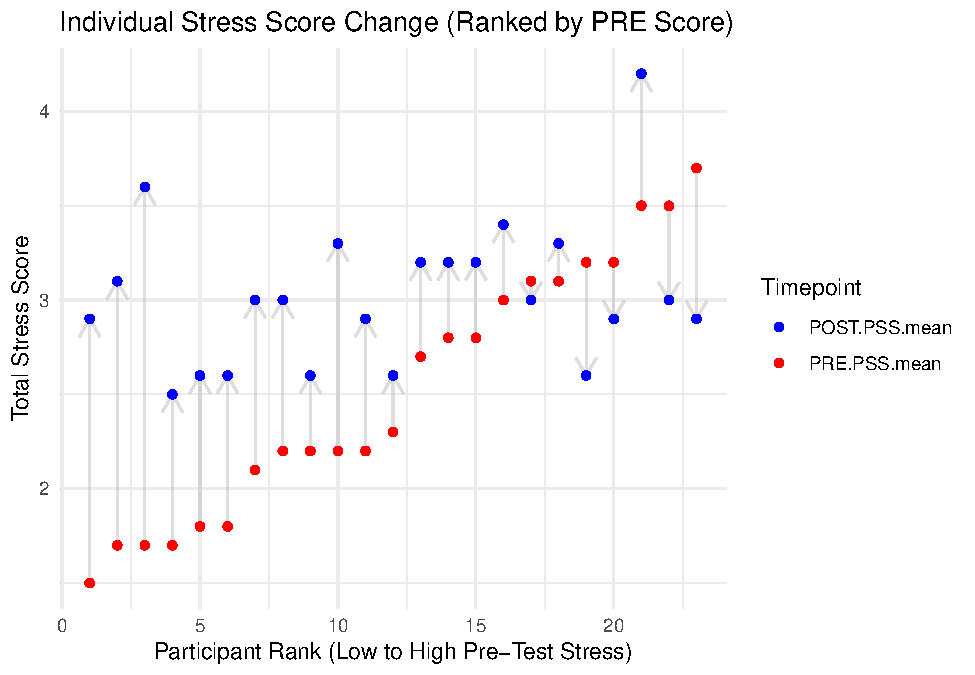
\includegraphics[keepaspectratio]{_plot_images/unnamed-chunk-10-1.pdf}}

\subsection{End PSS Section}\label{end-pss-section}

\subsubsection{-----------------}\label{section}

\section{EFF Section}\label{eff-section}

\subsection{Chunk 7: EFF Change Score Calculation \& Descriptive
Verification}\label{chunk-7-eff-change-score-calculation-descriptive-verification}

\begin{Shaded}
\begin{Highlighting}[]
\NormalTok{EFF\_analytic }\OtherTok{\textless{}{-}}\NormalTok{ EFF }\SpecialCharTok{|\textgreater{}} 
  \FunctionTok{mutate}\NormalTok{(}
    \AttributeTok{Group\_Assignment =} \FunctionTok{factor}\NormalTok{(Group\_Assignment),}
    \AttributeTok{EFF\_sum\_change   =}\NormalTok{ POST.EFF.sum }\SpecialCharTok{{-}}\NormalTok{ PRE.EFF.sum,}
    \AttributeTok{EFF\_mean\_change  =}\NormalTok{ POST.EFF.mean }\SpecialCharTok{{-}}\NormalTok{ PRE.EFF.mean}
    \CommentTok{\#Include\_Outliers = PRE.EFF.sum \textless{} 30}
\NormalTok{  )}

\CommentTok{\# Change{-}score descriptive table stratified by group}
\NormalTok{study.t1.change\_eff }\OtherTok{\textless{}{-}}\NormalTok{ EFF\_analytic }\SpecialCharTok{|\textgreater{}} 
  \CommentTok{\#filter(Include\_Outliers == TRUE) |\textgreater{} }
  \FunctionTok{CreateTableOne}\NormalTok{(}
    \AttributeTok{vars =} \FunctionTok{c}\NormalTok{(}\StringTok{"EFF\_sum\_change"}\NormalTok{, }\StringTok{"EFF\_mean\_change"}\NormalTok{),}
    \AttributeTok{strata =} \StringTok{"Group\_Assignment"}\NormalTok{,}
    \AttributeTok{testNormal =} \StringTok{"oneway.test"}
\NormalTok{  )}

\NormalTok{study.t1.change\_eff }\SpecialCharTok{|\textgreater{}} 
  \FunctionTok{print}\NormalTok{(}\AttributeTok{showAllLevels =} \ConstantTok{TRUE}\NormalTok{, }\AttributeTok{quote =} \ConstantTok{FALSE}\NormalTok{, }\AttributeTok{noSpaces =} \ConstantTok{TRUE}\NormalTok{) }\SpecialCharTok{|\textgreater{}} 
  \FunctionTok{kable}\NormalTok{(}\AttributeTok{caption =} \StringTok{"Efficacy (EFF) {-} Change Score Descriptive Table (Post {-} Pre)"}\NormalTok{) }\SpecialCharTok{|\textgreater{}} 
  \FunctionTok{kable\_styling}\NormalTok{(}\AttributeTok{bootstrap\_options =} \FunctionTok{c}\NormalTok{(}\StringTok{"striped"}\NormalTok{, }\StringTok{"hover"}\NormalTok{), }\AttributeTok{full\_width =} \ConstantTok{FALSE}\NormalTok{)}
\end{Highlighting}
\end{Shaded}

\begin{verbatim}
##                              Stratified by Group_Assignment
##                               level Control      Intervention p     test
##   n                                 5            23                     
##   EFF_sum_change (mean (SD))        -3.00 (6.86) 6.91 (24.91) 0.392     
##   EFF_mean_change (mean (SD))       -0.19 (0.43) 0.07 (0.62)  0.396
\end{verbatim}

\begin{longtable}[t]{llllll}
\caption{\label{tab:unnamed-chunk-11}Efficacy (EFF) - Change Score Descriptive Table (Post - Pre)}\\
\toprule
 & level & Control & Intervention & p & test\\
\midrule
n &  & 5 & 23 &  & \\
EFF\_sum\_change (mean (SD)) &  & -3.00 (6.86) & 6.91 (24.91) & 0.392 & \\
EFF\_mean\_change (mean (SD)) &  & -0.19 (0.43) & 0.07 (0.62) & 0.396 & \\
\bottomrule
\end{longtable}

\begin{itemize}
\tightlist
\item
  Average Change in Score for Groups.
\end{itemize}

\begin{Shaded}
\begin{Highlighting}[]
\DocumentationTok{\#\# {-}{-}{-}{-}{-}{-}{-}{-}{-}{-}{-}{-}{-}{-}{-}{-}{-}{-}{-}{-}{-}{-}{-}{-}{-}{-}{-}{-}{-}{-}{-}{-}{-}{-}{-}{-}{-}{-}{-}{-}{-}{-}{-}{-}{-}{-}{-}{-}{-}{-}{-}{-}{-}{-}{-}{-}{-}{-}{-}{-}{-}{-}{-}{-}{-}{-}{-}{-}{-}{-}{-}{-}{-}{-}{-}{-}{-}}
\CommentTok{\# Chunk 8: Within{-}Group Verification (Paired t{-}tests by Group)}
\DocumentationTok{\#\# {-}{-}{-}{-}{-}{-}{-}{-}{-}{-}{-}{-}{-}{-}{-}{-}{-}{-}{-}{-}{-}{-}{-}{-}{-}{-}{-}{-}{-}{-}{-}{-}{-}{-}{-}{-}{-}{-}{-}{-}{-}{-}{-}{-}{-}{-}{-}{-}{-}{-}{-}{-}{-}{-}{-}{-}{-}{-}{-}{-}{-}{-}{-}{-}{-}{-}{-}{-}{-}{-}{-}{-}{-}{-}{-}{-}{-}}
\NormalTok{EFF\_long }\OtherTok{\textless{}{-}}\NormalTok{ EFF\_analytic }\SpecialCharTok{|\textgreater{}} 
  \CommentTok{\#filter(Include\_Outliers == TRUE) |\textgreater{} \# This does not change the result}
  \FunctionTok{pivot\_longer}\NormalTok{(}
    \AttributeTok{cols =} \FunctionTok{c}\NormalTok{(PRE.EFF.mean, POST.EFF.mean),}
    \AttributeTok{names\_to =} \StringTok{"Time"}\NormalTok{,}
    \AttributeTok{values\_to =} \StringTok{"EFF\_mean"}
\NormalTok{  ) }\SpecialCharTok{|\textgreater{}} 
  \FunctionTok{mutate}\NormalTok{(}
    \AttributeTok{Time =} \FunctionTok{factor}\NormalTok{(}\FunctionTok{if\_else}\NormalTok{(}\FunctionTok{str\_detect}\NormalTok{(Time, }\StringTok{"PRE"}\NormalTok{), }\StringTok{"Pre"}\NormalTok{, }\StringTok{"Post"}\NormalTok{), }\AttributeTok{levels =} \FunctionTok{c}\NormalTok{(}\StringTok{"Post"}\NormalTok{, }\StringTok{"Pre"}\NormalTok{)) }\CommentTok{\# ifelse \textasciitilde{} Pre=TRUE, Post=FALSE, Pre==1, Post==0, levels = 0,1 (Post, Pre)}
\NormalTok{  )}

\NormalTok{eff\_paired\_tests }\OtherTok{\textless{}{-}}\NormalTok{ EFF\_long }\SpecialCharTok{|\textgreater{}} 
  \FunctionTok{group\_by}\NormalTok{(Group\_Assignment) }\SpecialCharTok{|\textgreater{}} 
  \FunctionTok{t\_test}\NormalTok{(EFF\_mean }\SpecialCharTok{\textasciitilde{}}\NormalTok{ Time, }\AttributeTok{paired =} \ConstantTok{TRUE}\NormalTok{, }\AttributeTok{detailed =} \ConstantTok{TRUE}\NormalTok{) }\SpecialCharTok{|\textgreater{}} 
  \FunctionTok{add\_significance}\NormalTok{()}

\NormalTok{eff\_paired\_tests }\SpecialCharTok{|\textgreater{}} 
  \FunctionTok{select}\NormalTok{(Group\_Assignment, estimate, conf.low, conf.high, statistic, df, p, p.signif) }\SpecialCharTok{|\textgreater{}} 
  \FunctionTok{kable}\NormalTok{(}\AttributeTok{caption =} \StringTok{"EFF mean Score {-} Within{-}Group Paired t{-}Tests"}\NormalTok{) }\SpecialCharTok{|\textgreater{}} 
  \FunctionTok{kable\_styling}\NormalTok{(}\AttributeTok{bootstrap\_options =} \FunctionTok{c}\NormalTok{(}\StringTok{"striped"}\NormalTok{, }\StringTok{"hover"}\NormalTok{), }\AttributeTok{full\_width =} \ConstantTok{FALSE}\NormalTok{)}
\end{Highlighting}
\end{Shaded}

\begin{longtable}[t]{lrrrrrrl}
\caption{\label{tab:unnamed-chunk-12}EFF mean Score - Within-Group Paired t-Tests}\\
\toprule
Group\_Assignment & estimate & conf.low & conf.high & statistic & df & p & p.signif\\
\midrule
Control & -0.188 & -0.720 & 0.345 & -0.978 & 4 & 0.383 & ns\\
Intervention & 0.067 & -0.203 & 0.337 & 0.515 & 22 & 0.612 & ns\\
\bottomrule
\end{longtable}

\begin{Shaded}
\begin{Highlighting}[]
\DocumentationTok{\#\# {-}{-}{-}{-}{-}{-}{-}{-}{-}{-}{-}{-}{-}{-}{-}{-}{-}{-}{-}{-}{-}{-}{-}{-}{-}{-}{-}{-}{-}{-}{-}{-}{-}{-}{-}{-}{-}{-}{-}{-}{-}{-}{-}{-}{-}{-}{-}{-}{-}{-}{-}{-}{-}{-}{-}{-}{-}{-}{-}{-}{-}{-}{-}{-}{-}{-}{-}{-}{-}{-}{-}{-}{-}{-}{-}{-}{-}}
\CommentTok{\# Chunk 9: Between{-}Group Models (ANCOVA \& Linear Mixed{-}Effects Model)}
\DocumentationTok{\#\# {-}{-}{-}{-}{-}{-}{-}{-}{-}{-}{-}{-}{-}{-}{-}{-}{-}{-}{-}{-}{-}{-}{-}{-}{-}{-}{-}{-}{-}{-}{-}{-}{-}{-}{-}{-}{-}{-}{-}{-}{-}{-}{-}{-}{-}{-}{-}{-}{-}{-}{-}{-}{-}{-}{-}{-}{-}{-}{-}{-}{-}{-}{-}{-}{-}{-}{-}{-}{-}{-}{-}{-}{-}{-}{-}{-}{-}}
\CommentTok{\# Model 1: ANCOVA (Predicting Post score controlling for Pre{-}score)}
\NormalTok{fit\_ancova\_eff }\OtherTok{\textless{}{-}} \FunctionTok{lm}\NormalTok{(POST.EFF.mean }\SpecialCharTok{\textasciitilde{}}\NormalTok{ PRE.EFF.mean }\SpecialCharTok{+}\NormalTok{ Group\_Assignment, }
                     \AttributeTok{data =}\NormalTok{ EFF\_analytic) }\CommentTok{\#|\textgreater{} filter(Include\_Outliers == FALSE))}
\FunctionTok{anova}\NormalTok{(fit\_ancova\_eff)}
\end{Highlighting}
\end{Shaded}

\begin{verbatim}
## Analysis of Variance Table
## 
## Response: POST.EFF.mean
##                  Df Sum Sq Mean Sq F value Pr(>F)   
## PRE.EFF.mean      1   2.80   2.798    9.41 0.0051 **
## Group_Assignment  1   0.12   0.117    0.39 0.5360   
## Residuals        25   7.43   0.297                  
## ---
## Signif. codes:  0 '***' 0.001 '**' 0.01 '*' 0.05 '.' 0.1 ' ' 1
\end{verbatim}

\begin{Shaded}
\begin{Highlighting}[]
\CommentTok{\# Model 2: Repeated Measures Linear Mixed{-}Effects (Group x Time interaction)}
\NormalTok{fit\_lmm\_eff }\OtherTok{\textless{}{-}} \FunctionTok{lmer}\NormalTok{(EFF\_mean }\SpecialCharTok{\textasciitilde{}}\NormalTok{ Group\_Assignment }\SpecialCharTok{*}\NormalTok{ Time }\SpecialCharTok{+}\NormalTok{ (}\DecValTok{1} \SpecialCharTok{|}\NormalTok{ Study\_ID), }
                    \AttributeTok{data =}\NormalTok{ EFF\_long) }\CommentTok{\# |\textgreater{} filter(Include\_Outliers == FALSE))}

\FunctionTok{anova}\NormalTok{(fit\_lmm\_eff)}
\end{Highlighting}
\end{Shaded}

\begin{verbatim}
## Analysis of Variance Table
##                       npar Sum Sq Mean Sq F value
## Group_Assignment         1 0.0173  0.0173    0.10
## Time                     1 0.0065  0.0065    0.04
## Group_Assignment:Time    1 0.1330  0.1330    0.79
\end{verbatim}

\begin{Shaded}
\begin{Highlighting}[]
\CommentTok{\# meanmary Outputs}
\FunctionTok{anova}\NormalTok{(fit\_ancova\_eff) }\SpecialCharTok{|\textgreater{}} 
\NormalTok{  broom}\SpecialCharTok{::}\FunctionTok{tidy}\NormalTok{() }\SpecialCharTok{|\textgreater{}} 
  \FunctionTok{kable}\NormalTok{(}\AttributeTok{caption =} \StringTok{"EFF mean {-} ANCOVA Model meanmary (Controlling for Pre{-}Score)"}\NormalTok{) }\SpecialCharTok{|\textgreater{}} 
  \FunctionTok{kable\_styling}\NormalTok{(}\AttributeTok{bootstrap\_options =} \FunctionTok{c}\NormalTok{(}\StringTok{"striped"}\NormalTok{, }\StringTok{"hover"}\NormalTok{), }\AttributeTok{full\_width =} \ConstantTok{FALSE}\NormalTok{)}
\end{Highlighting}
\end{Shaded}

\begin{longtable}[t]{lrrrrr}
\caption{\label{tab:unnamed-chunk-13}EFF mean - ANCOVA Model meanmary (Controlling for Pre-Score)}\\
\toprule
term & df & sumsq & meansq & statistic & p.value\\
\midrule
PRE.EFF.mean & 1 & 2.798 & 2.798 & 9.408 & 0.005\\
Group\_Assignment & 1 & 0.117 & 0.117 & 0.394 & 0.536\\
Residuals & 25 & 7.434 & 0.297 & NA & NA\\
\bottomrule
\end{longtable}

\begin{Shaded}
\begin{Highlighting}[]
\FunctionTok{anova}\NormalTok{(fit\_lmm\_eff) }\SpecialCharTok{|\textgreater{}} 
\NormalTok{  broom}\SpecialCharTok{::}\FunctionTok{tidy}\NormalTok{() }\SpecialCharTok{|\textgreater{}} 
  \FunctionTok{kable}\NormalTok{(}\AttributeTok{caption =} \StringTok{"EFF mean {-} Repeated Measures LMM ANOVA (Group * Time)"}\NormalTok{) }\SpecialCharTok{|\textgreater{}} 
  \FunctionTok{kable\_styling}\NormalTok{(}\AttributeTok{bootstrap\_options =} \FunctionTok{c}\NormalTok{(}\StringTok{"striped"}\NormalTok{, }\StringTok{"hover"}\NormalTok{), }\AttributeTok{full\_width =} \ConstantTok{FALSE}\NormalTok{)}
\end{Highlighting}
\end{Shaded}

\begin{longtable}[t]{lrrrr}
\caption{\label{tab:unnamed-chunk-13}EFF mean - Repeated Measures LMM ANOVA (Group * Time)}\\
\toprule
term & npar & sumsq & meansq & statistic\\
\midrule
Group\_Assignment & 1 & 0.017 & 0.017 & 0.103\\
Time & 1 & 0.007 & 0.007 & 0.039\\
Group\_Assignment:Time & 1 & 0.133 & 0.133 & 0.793\\
\bottomrule
\end{longtable}

\subsection{Effect Sizes}\label{effect-sizes}

\subsubsection{PSS}\label{pss}

\begin{Shaded}
\begin{Highlighting}[]
\FunctionTok{library}\NormalTok{(emmeans)}
\CommentTok{\# Partial eta{-}squared for ANCOVA}
\NormalTok{effectsize}\SpecialCharTok{::}\FunctionTok{eta\_squared}\NormalTok{(fit\_ancova, }\AttributeTok{partial =} \ConstantTok{TRUE}\NormalTok{) }\CommentTok{\#PSS}
\end{Highlighting}
\end{Shaded}

\begin{verbatim}
## # Effect Size for ANOVA (Type I)
## 
## Parameter        | Eta2 (partial) |       95% CI
## ------------------------------------------------
## PRE.PSS.mean     |           0.10 | [0.00, 1.00]
## Group_Assignment |       7.91e-03 | [0.00, 1.00]
## 
## - One-sided CIs: upper bound fixed at [1.00].
\end{verbatim}

\begin{Shaded}
\begin{Highlighting}[]
\CommentTok{\# Estimated Marginal Means (Adjusted Group Means at Post)}
\NormalTok{emmeans}\SpecialCharTok{::}\FunctionTok{emmeans}\NormalTok{(fit\_ancova, }\AttributeTok{specs =}\NormalTok{ pairwise }\SpecialCharTok{\textasciitilde{}}\NormalTok{ Group\_Assignment)}
\end{Highlighting}
\end{Shaded}

\begin{verbatim}
## $emmeans
##  Group_Assignment emmean     SE df lower.CL upper.CL
##  Control            3.10 0.1560 25     2.78     3.42
##  Intervention       3.02 0.0727 25     2.87     3.17
## 
## Confidence level used: 0.95 
## 
## $contrasts
##  contrast               estimate    SE df t.ratio p.value
##  Control - Intervention    0.077 0.172 25   0.446  0.6590
\end{verbatim}

\subsubsection{EFF}\label{eff}

\begin{Shaded}
\begin{Highlighting}[]
\CommentTok{\# Partial eta{-}squared for ANCOVA}
\NormalTok{effectsize}\SpecialCharTok{::}\FunctionTok{eta\_squared}\NormalTok{(fit\_ancova\_eff, }\AttributeTok{partial =} \ConstantTok{TRUE}\NormalTok{) }\CommentTok{\#EFF}
\end{Highlighting}
\end{Shaded}

\begin{verbatim}
## # Effect Size for ANOVA (Type I)
## 
## Parameter        | Eta2 (partial) |       95% CI
## ------------------------------------------------
## PRE.EFF.mean     |           0.27 | [0.06, 1.00]
## Group_Assignment |           0.02 | [0.00, 1.00]
## 
## - One-sided CIs: upper bound fixed at [1.00].
\end{verbatim}

\begin{Shaded}
\begin{Highlighting}[]
\CommentTok{\# Estimated Marginal Means (Adjusted Group Means at Post)}
\NormalTok{emmeans}\SpecialCharTok{::}\FunctionTok{emmeans}\NormalTok{(fit\_ancova\_eff, }\AttributeTok{specs =}\NormalTok{ pairwise }\SpecialCharTok{\textasciitilde{}}\NormalTok{ Group\_Assignment)}
\end{Highlighting}
\end{Shaded}

\begin{verbatim}
## $emmeans
##  Group_Assignment emmean    SE df lower.CL upper.CL
##  Control            5.35 0.245 25     4.85     5.86
##  Intervention       5.52 0.114 25     5.29     5.76
## 
## Confidence level used: 0.95 
## 
## $contrasts
##  contrast               estimate    SE df t.ratio p.value
##  Control - Intervention    -0.17 0.271 25  -0.628  0.5360
\end{verbatim}

\section{Plots}\label{plots}

\begin{Shaded}
\begin{Highlighting}[]
\NormalTok{EFF\_analytic }\SpecialCharTok{\%\textgreater{}\%} 
  \FunctionTok{filter}\NormalTok{(Group\_Assignment }\SpecialCharTok{==} \StringTok{"Intervention"}\NormalTok{) }\SpecialCharTok{|\textgreater{}} 
  \FunctionTok{arrange}\NormalTok{(PRE.EFF.mean) }\SpecialCharTok{\%\textgreater{}\%} 
  \FunctionTok{mutate}\NormalTok{(}
    \AttributeTok{Rank\_Order =} \FunctionTok{seq\_along}\NormalTok{(PRE.EFF.mean),}
    \AttributeTok{Pct\_Order =} \FunctionTok{percent\_rank}\NormalTok{(PRE.EFF.mean)}
\NormalTok{  ) }\SpecialCharTok{\%\textgreater{}\%} 
  \FunctionTok{ggplot}\NormalTok{(}\FunctionTok{aes}\NormalTok{(}\AttributeTok{x =}\NormalTok{ Rank\_Order)) }\SpecialCharTok{+}
  \CommentTok{\# 1. Add the arrows (vertical segments)}
  \FunctionTok{geom\_segment}\NormalTok{(}\FunctionTok{aes}\NormalTok{(}
    \AttributeTok{xend =}\NormalTok{ Rank\_Order, }
    \AttributeTok{y =}\NormalTok{ PRE.EFF.mean, }
    \AttributeTok{yend =}\NormalTok{ POST.EFF.mean}
\NormalTok{  ), }
  \AttributeTok{arrow =} \FunctionTok{arrow}\NormalTok{(}\AttributeTok{length =} \FunctionTok{unit}\NormalTok{(.}\DecValTok{35}\NormalTok{, }\StringTok{"cm"}\NormalTok{)), }\CommentTok{\# Adds the arrow head}
  \AttributeTok{color =} \StringTok{"gray"}\NormalTok{, }
  \AttributeTok{alpha =} \FloatTok{0.5}\NormalTok{) }\SpecialCharTok{+}
  
  \CommentTok{\# 2. Add the PRE points}
  \FunctionTok{geom\_point}\NormalTok{(}\FunctionTok{aes}\NormalTok{(}\AttributeTok{y =}\NormalTok{ PRE.EFF.mean, }\AttributeTok{color =} \StringTok{"PRE.EFF.mean"}\NormalTok{)) }\SpecialCharTok{+}
  
  \CommentTok{\# 3. Add the POST points}
  \FunctionTok{geom\_point}\NormalTok{(}\FunctionTok{aes}\NormalTok{(}\AttributeTok{y =}\NormalTok{ POST.EFF.mean, }\AttributeTok{color =} \StringTok{"POST.EFF.mean"}\NormalTok{)) }\SpecialCharTok{+}
  
  \CommentTok{\#4. Grouping...}
  \CommentTok{\#facet\_wrap(\textasciitilde{}Complete)+}
  
  \CommentTok{\# Formatting}
  \FunctionTok{scale\_color\_manual}\NormalTok{(}\AttributeTok{values =} \FunctionTok{c}\NormalTok{(}\StringTok{"PRE.EFF.mean"} \OtherTok{=} \StringTok{"red"}\NormalTok{, }\StringTok{"POST.EFF.mean"} \OtherTok{=} \StringTok{"blue"}\NormalTok{)) }\SpecialCharTok{+}
  \FunctionTok{labs}\NormalTok{(}
    \AttributeTok{title =} \StringTok{"Individual Self{-}Efficacy Score Change (Ranked by PRE Score)"}\NormalTok{,}
    \AttributeTok{x =} \StringTok{"Participant Rank (Low to High PRE Self{-}Efficacy)"}\NormalTok{,}
    \AttributeTok{y =} \StringTok{"Total Self{-}Efficacy Score"}\NormalTok{,}
    \AttributeTok{color =} \StringTok{"Timepoint"}
\NormalTok{  ) }\SpecialCharTok{+}
  \FunctionTok{theme\_minimal}\NormalTok{()}
\end{Highlighting}
\end{Shaded}

\pandocbounded{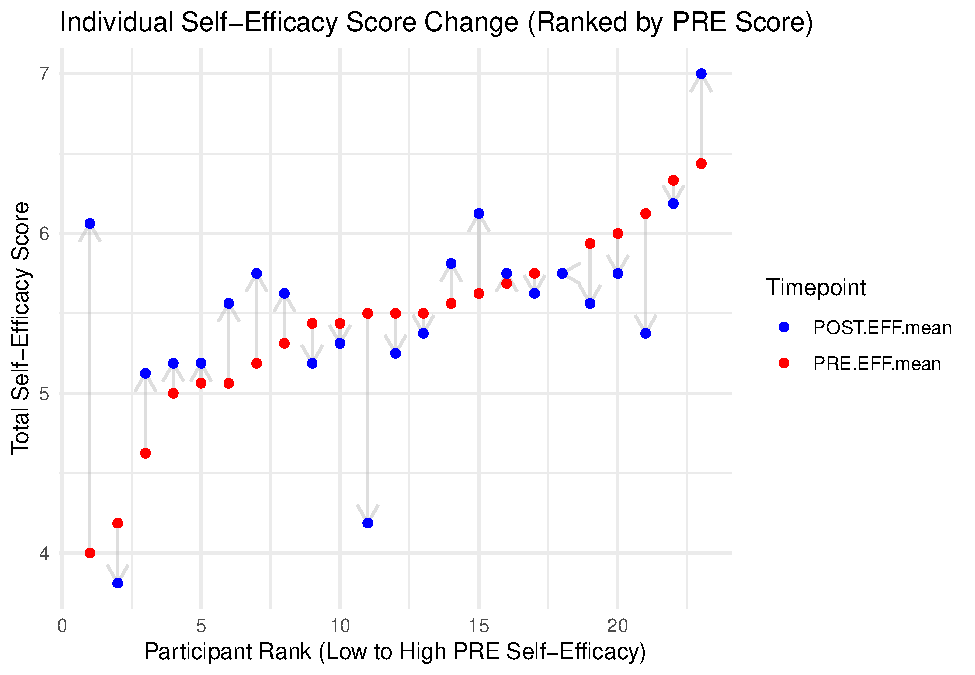
\includegraphics[keepaspectratio]{_plot_images/unnamed-chunk-16-1.pdf}}

\section{NOTES:}\label{notes}

\begin{itemize}
\tightlist
\item
  Efficacy Effects, Non-Significant, does not change with outlier
  screening.
\item
  Potentially needs a longer timescale of interaction.
\end{itemize}

\end{document}
